\chapter{Why Topology?}
\graphicspath{ {/home/tomasp/Dokumenty/Master_Thesis/figures/} }

Data has shape. This is hardly a new or revolutionary idea in the realm of data analysis and statistics. It is an assumption that we make all the time, even if we do not say it out loud. Whenever one tries to construct a linear regression model, we all have the mental image of a straight line in our minds, which should roughly approximate the data. This is then generalized via hyperplanes in higher dimensions.
\par
Another clear example would be periodic time series or signals -- we all expect to see a ``loop'' of some sort, given a long enough time interval between the measurements, see for example \ref{fig:SeattleWeather}.

\begin{figure}[h]
  \caption{Example plot of seasonal temperature changes in Seattle throughout the years.}
  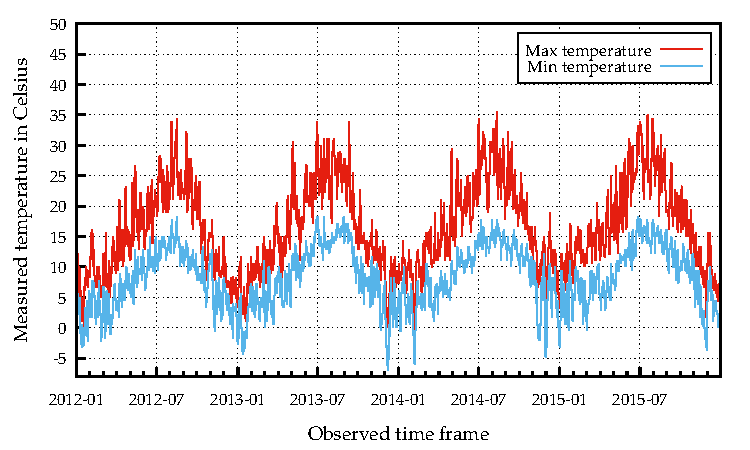
\includegraphics{weather.pdf}
  \centering
  \label{fig:SeattleWeather}
\end{figure}
